
\chapter{Øyesporing}

I dette kapittelet vil det bli gitt en kort innføring i hvordan øyet fungerer og hvordan det er mulig å spore dets bevegelser ved hjelp av en øyesporingsenhet. Til slutt vil det bli gitt en forklaring av øyesporingsenheten som brukes i dette prosjektet.

\section{Hvordan fungerer øyet?}

Å forklare hvordan øyet fungerer i detalj er utenfor denne rapportens omfang. Det vil derimot bli gitt en enkel forklaring av hvordan det fungerer og de mest nødvendige konseptene.

\subsection{Synsfelt}

I en artikkel skrevet av Tobii \cite{Calibration} sammenlignes øyet med et fotoapparat på grunn av deres mange likhetstrekk. Det hele starter ved at når lys treffer et objekt så reflekteres det og på samme måte som i et kamera fanges det reflekterte lyset opp av en linse. Dette blir så projisert på en lyssensitiv overflate, men i motsetning til i kamera, så er ikke denne overflaten like sensitiv overalt i øyet. Dette er fordi mennesker skal ha mulighet til å tilpasse synet etter hvor mye lys som er tilgjengelig. En bieffekt av dette er at en kun kan se klart i begrensede områder av synsfeltet. 

Dette fenomenet er illustrert i figur \ref{fig:visueltArea}, som viser hvordan synsfeltet hos mennesker er delt inn etter klarhet. Det innerste området notert ved bokstaven \textit{F} representerer det foveale området, også kjent som skarpsynet. Dette er den delen av synsfeltet man fokuserer på og som man derfor oppfatter som klarest. Det er hovedsakelig fra dette området visuell data hentes. Området deklarert med bokstavene \textit{Pf} i figuren viser det parafoveale området. Dette er et overgangsområde og kjennetegnes ved at uskarpheten gradvis øker til man kommer til det perifere området, vist som \textit{P} i figuren. Det perifere området, også kjent som sidesynet, er det mest uskarpe området og fungerer kun bra til å fange opp bevegelser og kontraster.

\begin{figure}[ht!]
\centering
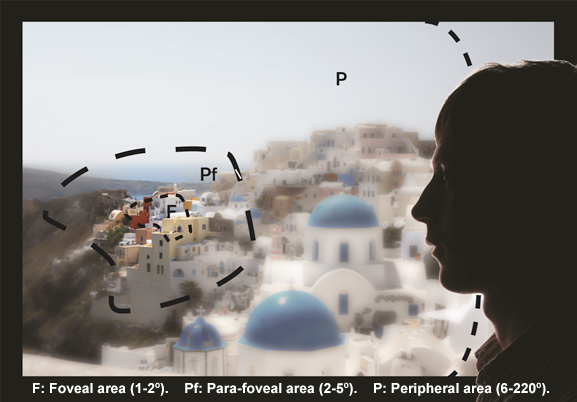
\includegraphics[width=80mm]{fovealArea}
\caption{Synsfeltet til et mennesker har forskjellige grader av skarphet. ( Hentet fra\cite{VisualImage})}
\label{fig:visueltArea}
\end{figure}

\subsection{Øyebevegelser}

Det foveale området er som tidligere nevnt det området hvor det registreres mest visuell data. Ulempen er at området kun står for rundt 2 grader av synsfeltet \cite{Backg0:online}. Så hvis en ønsker å hente detaljert informasjon fra andre deler av synsfeltet, må det foveale området flyttes ved å bevege øynene. Listen under, som er hentet fra Sansetap \cite{sanse7:online}, beskriver de ulike øyebevegelsene.


\subsubsection{Grovmotoriske}
\begin{itemize}
\item Akkomodasjon – øyets evne til å se klart på forskjellige avstander, det å kunne se skarpt når en flytter blikket hurtig fra avstand til nært og omvendt
\item Følgebevegelser – kunne følge en gjenstand med blikket i alle retninger uten å bevege hodet
\item Konvergens – kunne holde blikket samlet på nært hold
\item Stereosyn – evnen til å se avstand og dybde
\end{itemize}
\subsubsection{Finmotoriske}
\begin{itemize}
\item Sakkader – små forflytninger med blikket ved for eksempel lesing
\item Minisakkader – minibevegelser av øyet (dirring), som må være tilstede for at det skal sendes informasjon til hjernen
\item Antisakkader – evnen til å undertrykke en øyebevegelse
\item Fiksering – evnen til å holde blikket stødig festet på ett punkt
\end{itemize}



\section{Hva er øyesporing?}

Øyesporing er prosessen med å måle hvor en person ser, eller bevegelsen til et øye i forhold til hodet \cite{Eyet4:online}. Ved å gjøre dette kan man finne ut hvilke elementer brukeren ser på, hvor lenge han ser på dem og hvordan han beveger blikket. 


\subsection{Bruksområder}

Øyesporing kan anvendes på flere måter. Blant annet brukte Alfred L. Yarbus øyesporing til forskning. I sin artikkel fra 1967 \cite{wexle4:online} beskriver han hvordan et subjekts øyebevegelser påvirkes av oppgaven han skal gjennomføre. Bilde \ref{fig:yarbus} viser hvor forskjellig en person ser på et bilde basert på hvilken oppgave han er tildelt. I tillegg til vitenskap brukes øyesporing også til markedsundersøkelser, reklame, brukervennlighetstesting og mer \cite{Case2:online}. Det som kjennetegner de nevnte bruksområdene er at brukeren ikke aktivt foretar seg noe, han bruker ikke øynene til å gjøre noe annet enn å se. Det er annerledes enn anvendelsen i denne oppgaven, hvor øynene i tillegg til å se, brukes til interaksjon.

\begin{figure}[ht!]
\centering
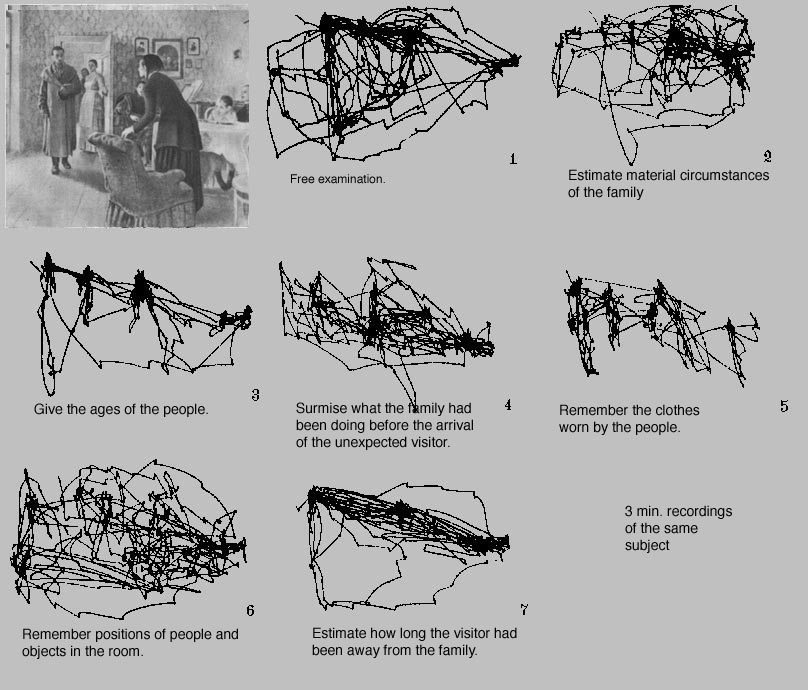
\includegraphics[width=100mm]{Yarbus_The_Visitor}
\caption{Hvilken oppgave en subjekt skal gjennomføre påvirker hans øyebevegelser \cite{Yarbu2:online}}
\label{fig:yarbus}
\end{figure}


\subsection{Pupil Centre Cornea Reflection}

Øyesporing er som tidligere nevnt teknikken brukt til å fange og måle øyebevegelser. For å gå til dette finnes det flere fremgangsmåter. I denne oppgaven vil det brukes en ikke-forstyrrende øyesporingsenhet. Dette gjør at brukeren i prinsippet ikke skal legge merke til enheten. 

\begin{figure}[ht!]
\centering
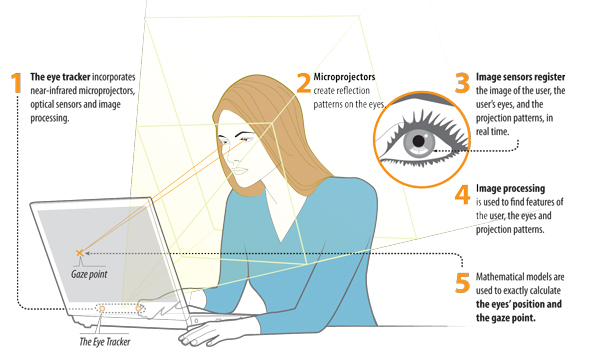
\includegraphics[width=120mm]{PCCR}
\caption{5 skritt som forklarer hvordan en øyesporingsenhet finner ut hvor en bruker ser på en monitor \cite{Under3:online}}
\label{fig:PCCR}
\end{figure}

For denne typen øyesporing er det mest vanlig å bruke en teknikk som heter Pupil Centre Cornea Reflection (\gls{PCCR}) \cite{Calibration}, som oversatt vil si midten av pupillen og hornhinnens refleksjon . Teknikken fungerer ved at en lyskilde belyser øyet for at refleksjonene skal bli klare og synlige. Et kamera tar et bilde av refleksjonene som øyet gir fra seg. Dette bildet blir så brukt til å identifisere lysets refleksjon på hornhinnen og pupillen. Når en vet vinkelen mellom hornhinnen og pupillen kan en regne ut blikkretningen og dermed hvor brukeren ser \cite{Calibration}.



\section{Tobii PCEye Go}

I prototypen har vi valgt å ta i bruk øyesporingsenheten Tobii PCeye GO \cite{Contr4:online}, vist i figur \ref{fig:tobiiPc}. Enheten kommer separat og kobles til datamaskinen via USB. Denne enheten ble valgt fordi den brukes i Sono Flex og fordi kontaktpersonen i Tobii allerede hadde god erfaring med enheten. Den har også den fordelen at den er av den ikke-forstyrrende typen, som vil si at en bruker i teorien ikke vil plages av enheten. Som ikke hadde vært tilfelle ved å tatt i bruk briller til øyesporing, som for eksempel  bildene vist i figur \ref{fig:tobii_glasses} .

\begin{figure}[ht!]
\centering
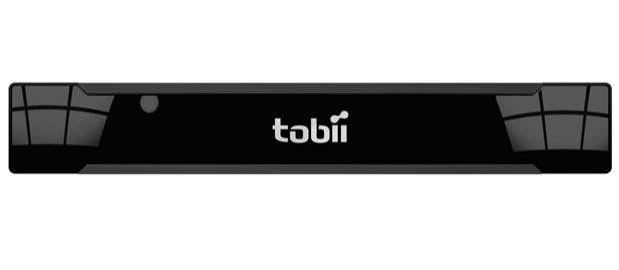
\includegraphics[width=50mm]{TobiiEyeGo}
\caption{Øyesporingsenheten Tobii PCEye Go}
\label{fig:tobiiPc}
\end{figure}

\begin{figure}[ht!]
\centering
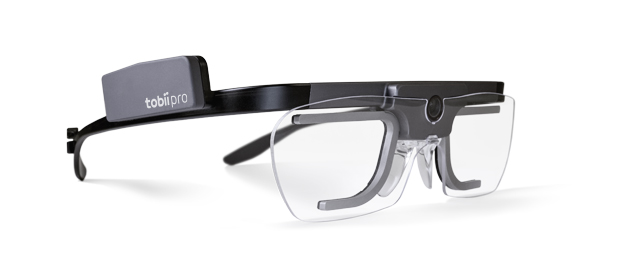
\includegraphics[width=50mm]{Tobii_Glasses}
\caption{Øyesporingsenhet i form av briller}
\label{fig:tobii_glasses}
\end{figure}


\subsection{Tobii Eye Control API }

Figur \ref{fig:overview} viser hvordan øyesporingsenheten eksponerer funksjonalitet til en klient-applikasjon gjennom APIet kalt TecAPI. For å ta det i bruk, tilbys to aksesspunkter. Det ene er gjennom .NET plattformen TecClient og det andre for C biblioteket MPACI.  Den praktiske betydningen er at man kun kan bruke APIet ved å skrive i enten C eller .NET teknologier. I denne rapporten vil kun sistnevnte være brukes, .NET APIet TecClient. 


\begin{figure}[ht!]
\centering
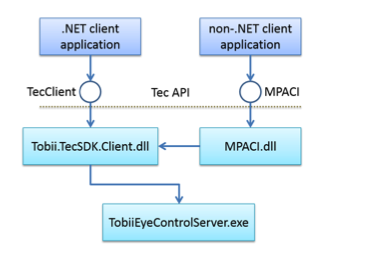
\includegraphics[width=100mm]{SoftwareArchitectureOverview}
\caption{Arkitekturen til blikkprogramvaren}
\label{fig:overview}
\end{figure}


\subsection{TecClient}

TecClient komponenten for .NET er delt inn i verktøysklasser(toolbox classes). Figur \ref{fig:toolbox} viser de ulike verktøyene som er tilgjengelig.

\begin{figure}[ht!]
\centering
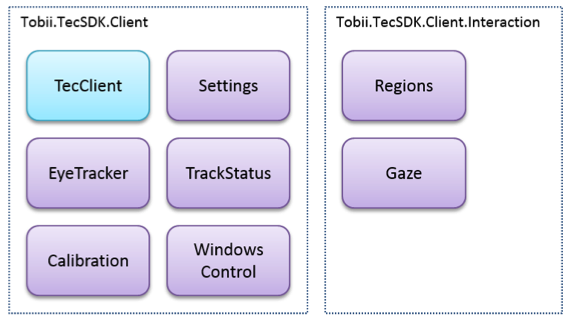
\includegraphics[width=100mm]{Toolbox}
\caption{Verktøyklasser som er tilgjengelige gjennom TecClient komponenten verktøyskasse}
\label{fig:toolbox}
\end{figure}


\subsubsection{EyeTracker} Gir informasjon om øyesporingsenheten. Som for eksempel om den er tilkoblet, hvilken brukerprofil som er aktiv og hvilken kalibreringsgrad den har.

\subsubsection{Calibration} 
Øyne oppfører seg forskjellig, så for at en øyesporingsenhet skal fungere optimalt må enheten kalibreres hver bruker.  Bilde \ref{fig:kalibre} viser et eksempel fra kalibreringsprosessen. I dette eksemplet blir brukeren bedt om å se på de ulike punktene. Mens brukeren gjør dette, samler øyesporingsenheten karakteristikk ved personens øyne. Karakteristikken brukes så til å lage en fysiologisk 3d modell av øyet som gjør at en vet hvordan brukerens øye oppfører seg \cite{www.t5:online}. 

\begin{figure}[ht!]
\centering
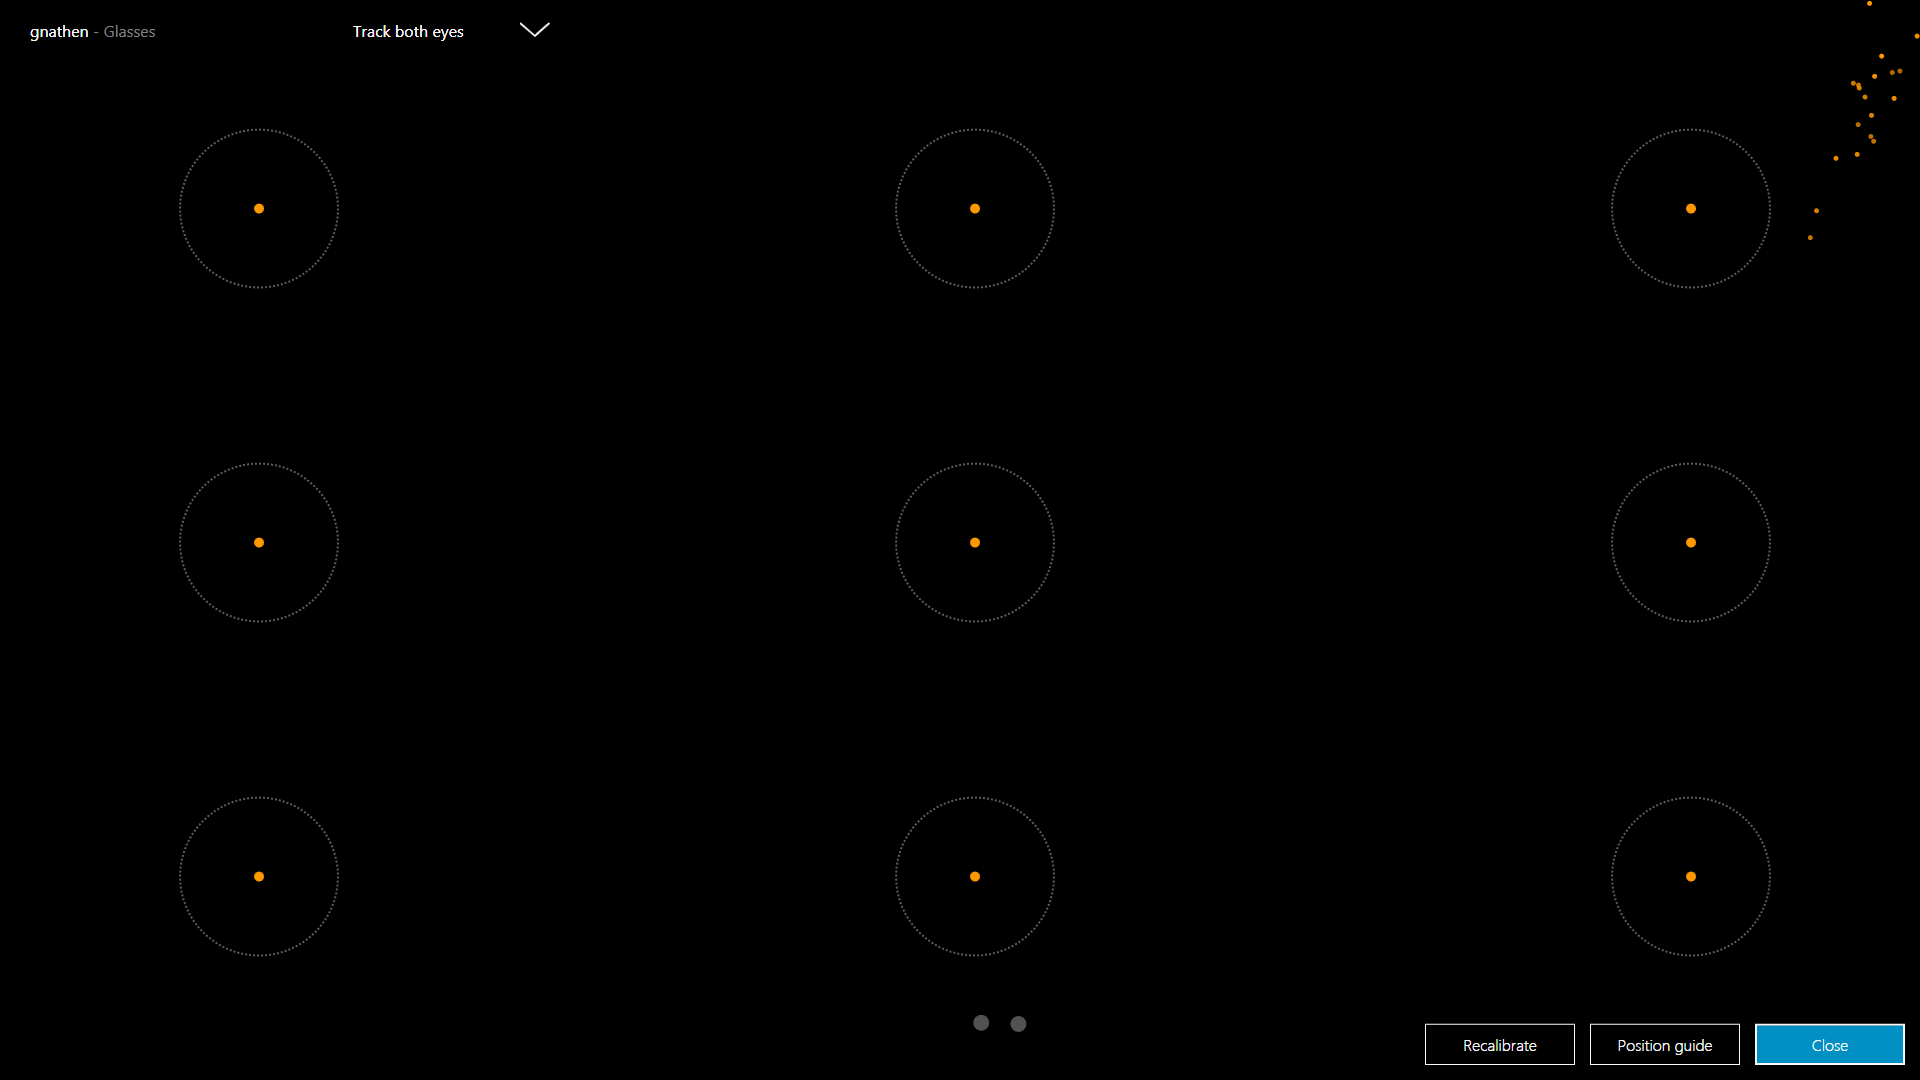
\includegraphics[width=100mm]{kalibrering}
\caption{Ni punkter som en bruker blir bedt om å se på for at øyesporingsenheten skal kunne kalibreres \cite{VHye88:online}}
\label{fig:kalibre}
\end{figure}


\subsubsection{Settings}
Settings-komponenten gir tilgang til brukerprofiler og operasjoner som gjør at man kan lage nye profilet og skifte mellom dem. For eksempel er det naturlig at en bruker ikke vil gå gjennom kalibreringsprosedyren hver gang han vil ta i bruk enheten. I denne komponenten kan karakteristikken fra kalibreringen lagres i brukerprofilen som er koblet til brukeren, slik at han slipper dette. 


\subsubsection{Trackstatus}
Trackstatus-komponenten tilbyr metoder, egenskaper og hendelser for å kontrollere sporingsstatus vinduet. Bilde \ref{fig:track} viser hvordan det kan brukes til å vise brukeren om enheten fanger opp øynene og hvordan hodet er plassert i forholdt til øyesporingsenheten.

\begin{figure}[ht!]
\centering
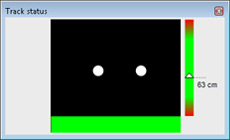
\includegraphics[width=100mm]{Trackstatus}
\caption{Eksempel på hvordan en bruker kan bli opplyst om øynene blir fanget opp og hvordan hodet er plassert i forhold til øyesporingsenheten}
\label{fig:track}
\end{figure}

\subsubsection{Gaze}
Gaze-komponenten eksponerer rå blikkdata, både filtrert og ufiltrert. Det vil si at man kan finne ut hvor på skjermen en bruker ser i form av x- og y-koordinater.  


\subsubsection{Region / Interaction regions}

Ifølge dokumentasjonen er en interaksjonregion en geometrisk region på skjermen som en bruker kan interagere ved å se på den (dokumentasjon). Hvis øynene ser innenfor en slik region vil applikasjonen bli opplyst om det. Knapper er et typisk eksempel på elementer som vil bli definert som interaksjonregioner, ettersom en bruker må ”trykke” på disse ved å bruke øynene. 

Ved å definere en slik region kan man lytte til hendelser fra dem. De to viktigste hendelsene er \textbf{Focus} og \textbf{Activation}. Focus-hendelsen vil aktiveres når en bruker skuer innenfor grensene til en region. En bruker vil bli opplyst om at han er innenfor en slik region ved hjelp av en indikator. Denne indikatoren vil typisk gi brukeren et signal om at en nedtelling har startet. Når nedtellingen er ferdig vil Activation-hendelsen bli kjørt. Activation er konseptuelt det samme som å klikke med en datamus, og responsen vil normalt være den samme.  




